\section{Cell Merge}\label{des:sec:merge}
The cell merge process is iterative and is dependent on the total sum of the error of the cells, $E$. Initially, this error is relatively low as multiple cells are generated with one or very few sources contained in each cell. To keep the maximum error threshold relative, unless it is given as an input by the user, it is calculated as the product of the set standard deviation ($\sigma$), the size of the plane ($x_{plane},y_{plane}$) and the number of sources in the plane ($|S|$) or 
\begin{equation}\label{des:eq:maxerr}
 E_{max} = \sigma x_{plane}y_{plane}|S|.
\end{equation}
The process begins by summing the errors of the cells and iterates through the process of finding the best merge, checking if implementing the best merge exceeds the maximum error threshold and, if not, implementing the best merge.

\subsection{Obtaining the Best Merge}
The best merge is obtained by iterating over the list of centres and, for each centre, testing it with its active neighbouring centres.
\\
\\
The merge test works by calculating a new centre, $c_{new} = (\vec{X},Z)$, determined by two existing centres, $c_1$ and $c_2$, with intensities $z_1$ and $z_2$, and positions $\vec{x_1}$ and $\vec{x_2}$, respectively, as
\begin{equation} \label{eq:merge_centre}
	\vec{X} = t\vec{x_1} + (1-t)\vec{x_2} \text{  with  } t = \frac{z_1}{z_1 + z_2}.
\end{equation}
The new weight for the merged centre is defined as
\begin{equation}
	Z = z_1 + z_2.
\end{equation}
Since $x_1$ and $x_2$ are centred sums of the positions of the sources in their cells, expanding them to their original forms yields
\begin{equation*}
\vec{x_1} = \frac{\sum^N_{i=1} z_{1i}\vec{x_{1i}}}{\sum^N_{i=1}z_{1i}} \text{  and  } \vec{z_2} = \frac{\sum^M_{i=1} z_{2i}\vec{x_{2i}}}{\sum^M_{i=1}z_{2i}}.
\end{equation*}
Note that:
\begin{equation*}
	z_j = \sum^N_{i=1}z_{ji}.
\end{equation*}
Substituting these into Equation (\ref{eq:merge_centre}), we obtain
\begin{align*}
	\vec{X}	&= t\vec{x_1} + (1-t)\vec{x_2} \\
		&= \frac{z_1}{z_1 + z_2}\frac{\sum^N_{i=1} z_{1i}\vec{x_{1i}}}{z_1} + (\frac{z_1 + z_2}{z_1 + z_2} - \frac{z_1}{z_1 + z_2})\frac{\sum^M_{i=1} z_{2i}\vec{x_{2i}}}{z_2} \\
		&= \frac{\sum^N_{i=1} z_{1i}\vec{x_{1i}}}{z_1 + z_2} + \frac{\sum^M_{i=1} z_{2i}\vec{x_{2i}}}{z_1 + z_2} \\
		&= \frac{\sum^N_{i=1} z_{1i}\vec{x_{1i}} + \sum^M_{i=1} z_{2i}\vec{x_{2i}}}{z_1 + z_2} \\
		&= \frac{\sum^N_{i=1} z_{1i}\vec{x_{1i}} + \sum^M_{i=1} z_{2i}\vec{x_{2i}}}{\sum^N_{i=1}z_{1i} + \sum^M_{i=1}z_{2i}}.
\end{align*}
This shows that Equation (\ref{eq:merge_centre}) is equivalent to finding the centre of all the sources in both $x_1$ and $x_2$.
\\
\\
Once the new centre has been found, the error must be determined by summing the square of the weighted distances to the new centre from each source. Once determined, the new centres coordinates and intensity, as well as the new error are returned. The error itself is not compared to find the best merge, but rather the change in error, that is, the merge that produces the lowest increase in the error. This is done by taking the tested merge error and subtracting from it the errors of the centres used to generate it; i.e., we seek $\Delta_{i,j}$ such that for some cells $c_i$ and $c_2j$, the comparison with the error of the merged cell, $c_{i,j}$ is:
\begin{equation}\label{des:eq:delta}
	\Delta_{i,j} = \min^n_{i = 1}\min^n_{j = 1, i \neq j}c_{i,j} - (c_i + c_j).
\end{equation}
Once found, the result is stored along with the new coordinates of the centre, $c_{i,j}$ and the centres used to generate it.
\\
\\
Once the best merge has been found, it must be determined whether the new sum of errors exceeds the threshold, i.e. $E + \Delta_{i,j} \geq E_{max}$. If it does, the merge process is halted and the Voronoi structure is returned. If the threshold is set too high, it may occur that all the cells merge into a single cell. In this case, the process is again halted as no best merge could be found as the threshold was set too high for the system. The Voronoi structure is returned as only the set of sources and a single centre with no bisecting lines remaining and so no merged Voronoi can be generated. If the system finds a valid merge which is still less than the threshold, it adds the difference in the merge error to the total error and executes the merge.

\subsection{Executing the Merge}
The merge execution algorithm takes in the new coordinates and intensity, $\vec{X}$, the new error, $Z$, as well as the centre, $c_1$, and the related centre with which it is to be merged, $c_2$. The algorithm starts by setting the coordinates and intensity of $c_1$ to those of $c_{1,2} = (\vec{X},Z)$. It deprecates the line relating $c_1$ to $c_2$ and appends the list of sources in $c_2$ to that of $c_1$. The error of $c_1$, $z_1$, is set to that of the new error, $Z$. Centre $c_2$ and its list of consumed centres are added to the list of consumed centres of $c_1$. Finally, the list of centres is iterated over and any centre which references $c_2$ is changed to reference $c_1$ and all lines which relate other centres to $c_2$ are changed to relate to $c_1$ instead. Once this is complete, the process of finding the best merge restarts until the error threshold is reached.
\\
\\
The transition from Figure \ref{fig:1merge1} to Figure \ref{fig:1merge2} shows the effects of a single merge. The weighted distance between the merged centres in Figure \ref{fig:1merge1} is less than those of all other neighbouring centre pairs.
\begin{figure}[H]
  \centering
  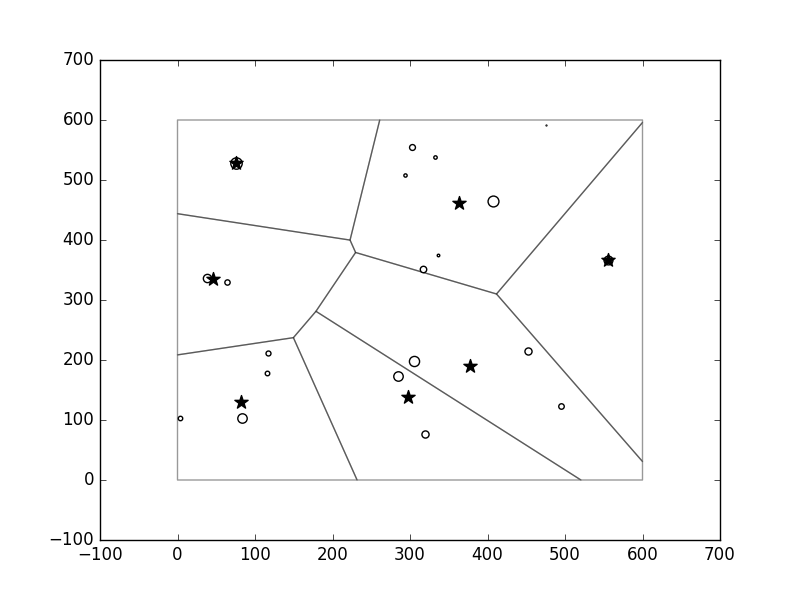
\includegraphics[width=0.8\textwidth]{Images/1merge1.png}
  \caption{Re-centred Voronoi before merge.}
  \label{fig:1merge1}
\end{figure}
\begin{figure}[H]
\centering
  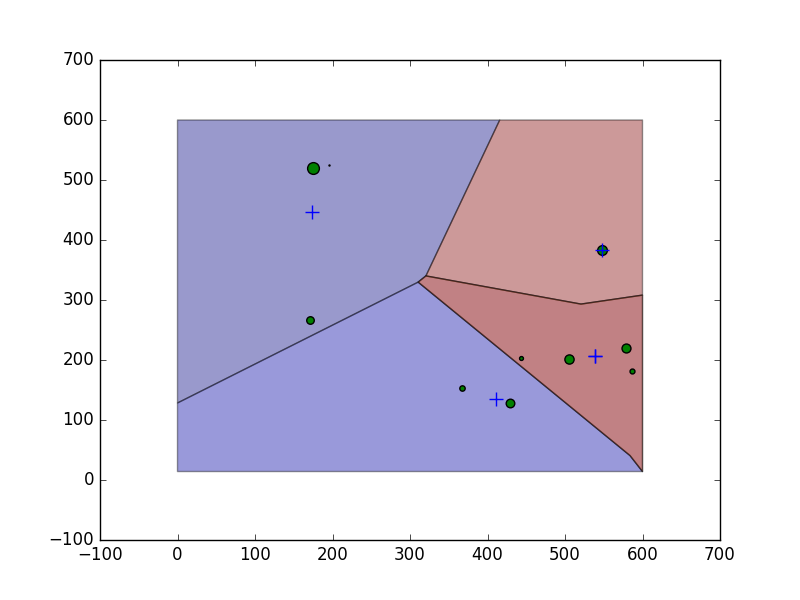
\includegraphics[width=0.8\textwidth]{Images/1merge2.png}
  \caption{Re-centred Voronoi after single merge.}
  \label{fig:1merge2}
\end{figure}
\begin{figure}[H]
\centering
  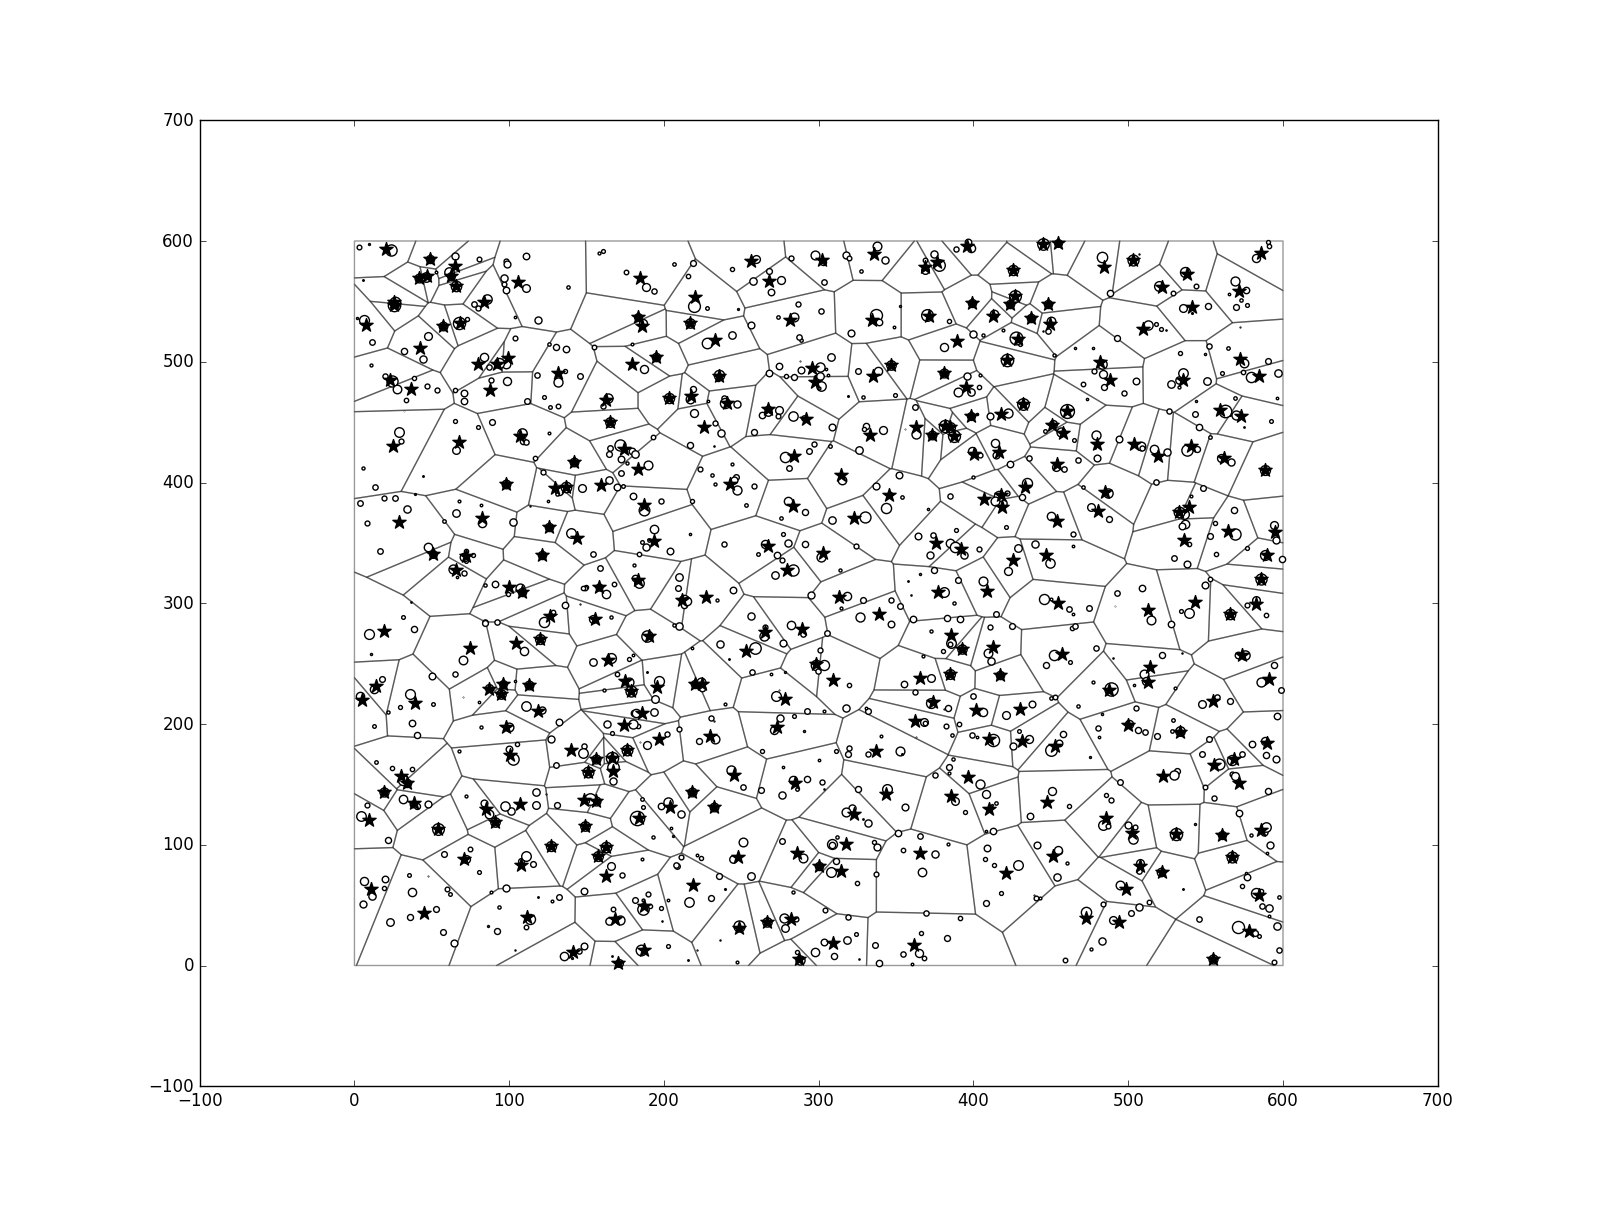
\includegraphics[width=0.8\linewidth]{Images/merge1.png}
  \caption{Re-centred Voronoi with 1000 sources and 301 centres before merge.}
  \label{fig:merge1}
\end{figure}
\begin{figure}[H]
\centering
  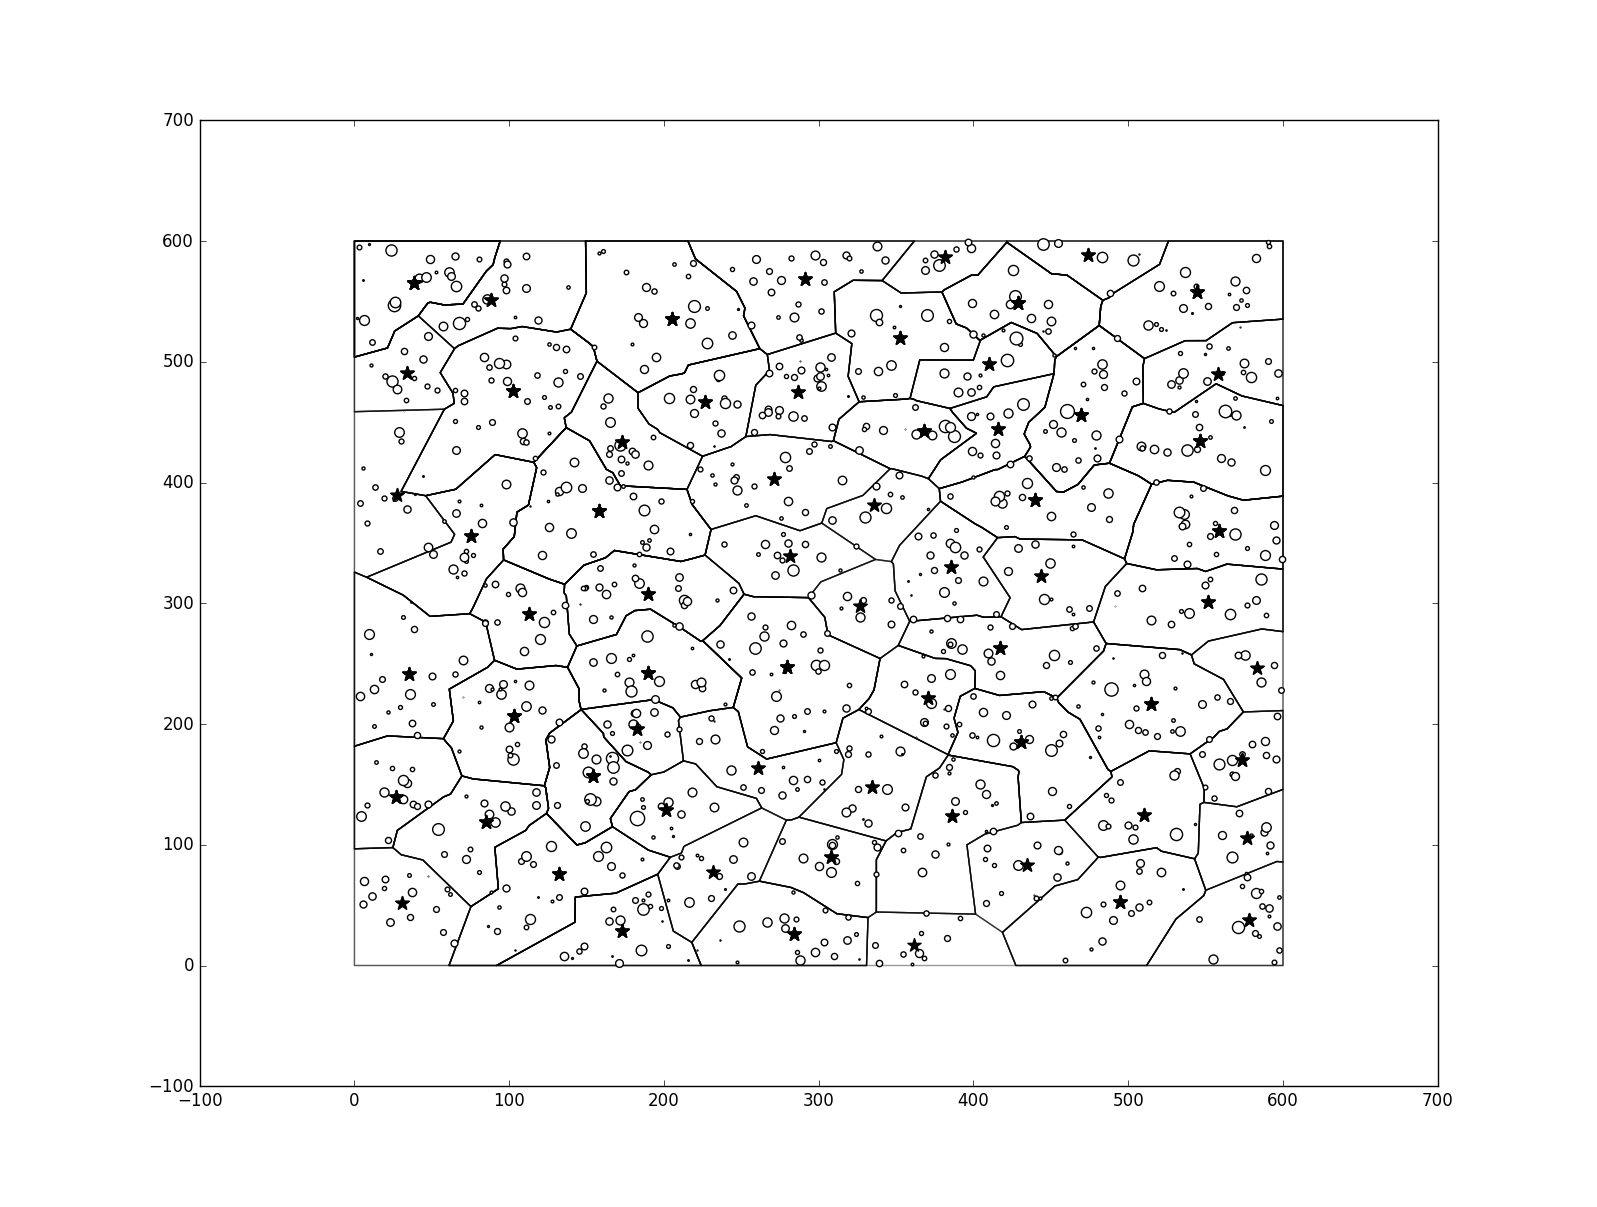
\includegraphics[width=0.8\linewidth]{Images/merge2.png}
  \caption{Re-centred Voronoi with 1000 sources and 64 centres after completing the merge process.}
  \label{fig:merge2}
\end{figure}
Figure \ref{fig:merge1} shows an initial Voronoi tessellation while Figure \ref{fig:merge2} shows its merged structure once the error threshold has been reached. The latter figure has larger structures with cells generally being more convex depending on the layout of sources in the cell.